\section{Experiments}
\label{sec:experiments}









Our experiments are designed to answer the following questions: 
\textbf{Q1:} Can LARM effectively learn dynamics from human-only videos and generalize to out-of-domain robotic embodiments? 
\textbf{Q2:} Does the intent-aligned latent residual improve downstream policy learning compared to static representations and unconstrained predictive models?
\textbf{Q3:} How does LARM perform across diverse policy architectures?


\subsection{Analysis of pre-trained representations}
\label{sec:exp_visualization}
We first investigate whether LARM successfully learns to extract intent-aligned dynamics during the human-video pre-training phase.

\noindent\textbf{Pre-training details.} 
We pre-train LARM strictly on human-centric videos using the Kinetics-400 training split~\cite{kay2017kinetics, carreira2017quo}, without any in-domain robotic manipulation data. To construct the dataset for our prediction-based self-supervised learning, we sample pairs of frames from each video. Specifically, we select the $1^{\text{st}}$ frame as the initial observation and the $96^{\text{th}}$ frame as the target future state. This specific temporal gap ($k=96$) is chosen to capture meaningful, long-horizon state transitions rather than trivial, high-frequency motions, as in~\cite{kim2025token}. \rev{Kinetics-400 is stored at $25$--$30$\,fps, so $k=96$ spans roughly $3$--$4$ seconds of human activity. The gap has to be large enough that the transition is not dominated by encoding noise: frames a fraction of a second apart are near-identical under a frozen DINOv3 encoder, so the prediction target would degenerate towards an identity map and the resulting residual would carry little task signal. We stress that $k$ is a hyper-parameter of pre-training on web video and \emph{not} a control horizon; at deployment the predictor is executed at every control step and its output is consumed as a direction, with magnitude and time scale absorbed by the action decoder (Sec.~\ref{subsec:deployment}).}
We adopt DINOv3 (ViT-Base/16)~\cite{simeoni2025dinov3}  as our foundational visual backbone, and DistilBERT-Base-Uncased~\cite{sanh2019distilbert} as the text backbone. To provide stable and high-quality latent targets without pixel-level reconstruction, as depicted in Fig.~\ref{fig:ab_probe}, we employ self-distillation on our visual backbone and formalize a frozen, pre-trained DINOv3 model as a  \textit{Teacher} model~\cite{grill2020bootstrap, caron2021emerging}. Simultaneously, our trainable LARM modules process the initial frame with the language instruction to predict this latent future and optimize the loss $\mathcal{L}_{\text{total}}$ defined in Eq.~\ref{eq:total}. 


% \begin{table*}[t]
% \centering
% \caption{\textbf{Results on Franka Kitchen~\cite{franka_kitchen}}. We classify the compared methods into three groups. To ensure a fair comparison, we use the most common pre-training dataset (Kinetics-300K) and model scale (ViT-Base) across all evaluations in this downstream, highlighting the effectiveness of our model design.}
% \setlength{\tabcolsep}{3pt}
% \resizebox{\textwidth}{!}{%
% \renewcommand{\arraystretch}{1.0}
% \begin{tabular}{@{}lllcccccc@{}}
% \toprule
% \bf Method &
% \bf  Backbone &
% \bf  Pre-training dataset  &
%   Turn knob &
%   Open door &
%   Flip switch &
%   Open microwave &
%   Slide door &
% \bf  Average \\ 




%   \midrule
% \rowcolor[HTML]{EFEFEF} 
%   \multicolumn{10}{l}{\cellcolor[HTML]{EFEFEF}Robotics-focused Vision-Language Models}                             \\ \midrule
% INSUP~\cite{insup}    & ResNet50                     & ImageNet~\cite{imagenet}         & 28.0 & 18.0 & 50.0 & 26.7 & 75.7  & 39.7  \\
% R3M~\cite{r3m}      & ResNet50                     & Ego4D~\cite{ego4d}             & 53.3 & 50.7 & 86.3 & 59.3 & 97.0  & 69.5  \\
% MVP~\cite{mvp1}      & ViT-Base                     & Multi-dataset   & 79.0 & 48.0 & 90.7 & 41.0 & \bf 100.0 & 71.7  \\
% Voltron~\cite{voltron} &
%   ViT-Base &
%   Something-Something~\cite{something2something} &
  
%   76.0 &
%   45.3 &
%   91.0 &
%   41.0 &
%   99.3 &
%   70.5 \\
% MPI~\cite{mpi}      & ViT-Base                     & Ego4D Hand-Obj~\cite{ego4d}   & 89.0 & \bf 57.7 & 93.7 & 54.0 & \bf 100.0 & 78.9  \\

% LaVA-Man~\cite{lava-man} & ViT-Base                     & Multi-dataset   &  90.0 & 50.7 &    94.0 &  61.3 & \bf 100.0 &  79.2  \\




% \midrule
%   \multicolumn{10}{l}{\cellcolor[HTML]{EFEFEF}General-purpose Vision-only Models}                             \\ \midrule

% CLIP~\cite{clip}   & ResNet50                     & Internet scale  & 26.3 & 13.0 & 41.7 & 24.7 & 86.3  & 38.4  \\
% SigLIP-1~\cite{siglip} &
%   \multicolumn{1}{l}{ViT-Base} &
%   Internet scale &
  
%   25.5 &
%   15.5 &
%   38.0 &
%   20.0 &
%   82.0 &
%   36.2 \\ 
% SimCLR~\cite{simclr}   & \multicolumn{1}{l}{ResNet50} &                &       25.3 & 72.3 & 55.8 & 23.3 & 72.3  & 49.8  \\
% MoCo v3~\cite{mocov3}  &                              &                &      11.5 & 66.5 & 24.3 & 14.3 & 66.5  & 36.6 \\
% DINO~\cite{dino}     &                              &                   & 27.0 & 77.0 & 44.3 & 28.5 & 77.0  & 50.8 \\
% MAE~\cite{heMasked2022}      &                              &                    & 12.0 & 71.5 & 24.3 & 10.0 & 71.5  & 37.9 \\
% SiamMAE~\cite{guptaSiamese2023}  &                              &                  & 16.8 & 68.0 & 36.5 & 13.5 & 68.0  & 40.6 \\
% RSP~\cite{rsp}      &                              &                 & 31.0 & 82.5 & 44.5 & 10.3 & 82.5  & 50.2 \\
% CropMAE~\cite{cropmae}  &                              &                  & 31.5 & 77.0 & 54.0 & 32.5 & 77.0  & 54.4  \\
% I-JEPA~\cite{i-jepa}   &                              &                  & 26.0 & 21.3 & 40.0 & 17.3 & 74.7  & 35.9 \\
% V-JEPA~\cite{v-jepa}   &                              &                  & 21.3 & 28.0 & 41.3 & 12.7 & 78.7  & 36.4  \\
% ToBo~\cite{kim2025tobo} &
%   \multirow{-10}{*}{ViT-Base} &
%   \multirow{-10}{*}{Kinetics}  &
%   57.0 &
%   51.0 &
%   82.0 &
%   55.0 &
%   95.0 &
%   68.0 \\

% DINOv3  &  ViT-Base  & Internet scale   &  79.3 &
% 43.7 &
% 92.3 &
% 40.3 &
% \bf 100.0 &
% 71.3 \\
  

% \rowcolor[HTML]{ECF4FF} 
% Ours     & ViT-Base                     & Internet scale, Kinetics  	& \bf 91.7 &  56.7 &	\bf 95.7 & \bf 62.0	& \bf 100.0	& \bf 81.2  \\


% % \rowcolor[HTML]{EFEFEF} 
%  \bottomrule
% \end{tabular}%
% }
% \label{tab:franka_kit_results}
% \end{table*}




\begin{table*}[!t]
\centering
\caption{\textbf{Results on Franka Kitchen~\cite{franka_kitchen}}. We report average success rates over 25 demonstrations across five tasks, two viewpoints, and three random seeds. All rows use the same frozen-backbone behavioral-cloning downstream and evaluation protocol, while the backbone and pre-training dataset columns expose the upstream data/model differences. Baselines are grouped by representation paradigm; success rates are reported in percent and the best result in each task column is bolded.}
\setlength{\tabcolsep}{3pt}
\resizebox{\textwidth}{!}{%
\renewcommand{\arraystretch}{1.0} 
\begin{tabular}{lllcccccc}
\toprule
\bf Method &
\bf Backbone &
\bf Pre-training dataset &
 Turn knob &
 Open door &
 Flip switch &
 Open microwave &
 Slide door &
\bf Average \\ 

\midrule

\rowcolor[HTML]{EFEFEF} 
\multicolumn{9}{l}{\textit{Visual Representation Models} } \\ 
DINOv3~\cite{simeoni2025dinov3}       & ViT-Base & Internet scale      & 79.3 & 43.7 & 92.3 & 40.3 & \bf 100.0 & 71.3 \\
R3M~\cite{nair2022r3m}                & ResNet50 & Ego4D~\cite{grauman2022ego4d}  & 53.3 & 50.7 & 86.3 & 59.3 & 97.0 & 69.5 \\
MVP~\cite{radosavovic2023real}        & ViT-Base & Multi-dataset       & 79.0 & 48.0 & 90.7 & 41.0 & \bf 100.0 & 71.7 \\

\midrule
% 同样去掉 [0pt][0pt] 和 @{}
\rowcolor[HTML]{EFEFEF} 
\multicolumn{9}{l}{\textit{Vision-only Predictive Models}} \\ 
SiamMAE~\cite{gupta2023siamese}       & ViT-Base & Kinetics~\cite{kay2017kinetics} & 16.8 & 68.0 & 36.5 & 13.5 & 68.0 & 40.6 \\
V-JEPA~\cite{bardes2024revisiting}             & ViT-Base & Kinetics & 21.3 & 28.0 & 41.3 & 12.7 & 78.7 & 36.4 \\
ToBo~\cite{kim2025token}              & ViT-Base & Kinetics & 57.0 & 51.0 & 82.0 & 55.0 & 95.0 & 68.0 \\

\midrule
% 同样去掉 [0pt][0pt] 和 @{}
\rowcolor[HTML]{EFEFEF} 
\multicolumn{9}{l}{\textit{Vision-Language Predictive Models} } \\ 
Voltron~\cite{karamcheti2023language} & ViT-Base & Something-V2~\cite{goyal2017something} & 76.0 & 45.3 & 91.0 & 41.0 & 99.3 & 70.5 \\
MPI~\cite{zeng2024learning}           & ViT-Base & Ego4D Hand-Obj~\cite{grauman2022ego4d} & 89.0 & \bf 57.7 & 93.7 & 54.0 & \bf 100.0 & 78.9 \\
LaVA-Man~\cite{zhu2025lava}           & ViT-Base & OOPP~\cite{zhu2025lava}, DROID~\cite{khazatsky2024droid}, Bridge~\cite{walke2023bridgedata}       & 90.0 & 50.7 & 94.0 & 61.3 & \bf 100.0 & 79.2 \\


\rowcolor[HTML]{DCD5E0} 
\textbf{Ours} & ViT-Base & Internet scale, Kinetics & \bf 91.7 & 56.7 & \bf 95.7 & \bf 62.0 & \bf 100.0 & \bf 81.2 \\

\bottomrule
\end{tabular}%
}
\label{tab:franka}
\end{table*}



\begin{figure}[t]  
    \centering
    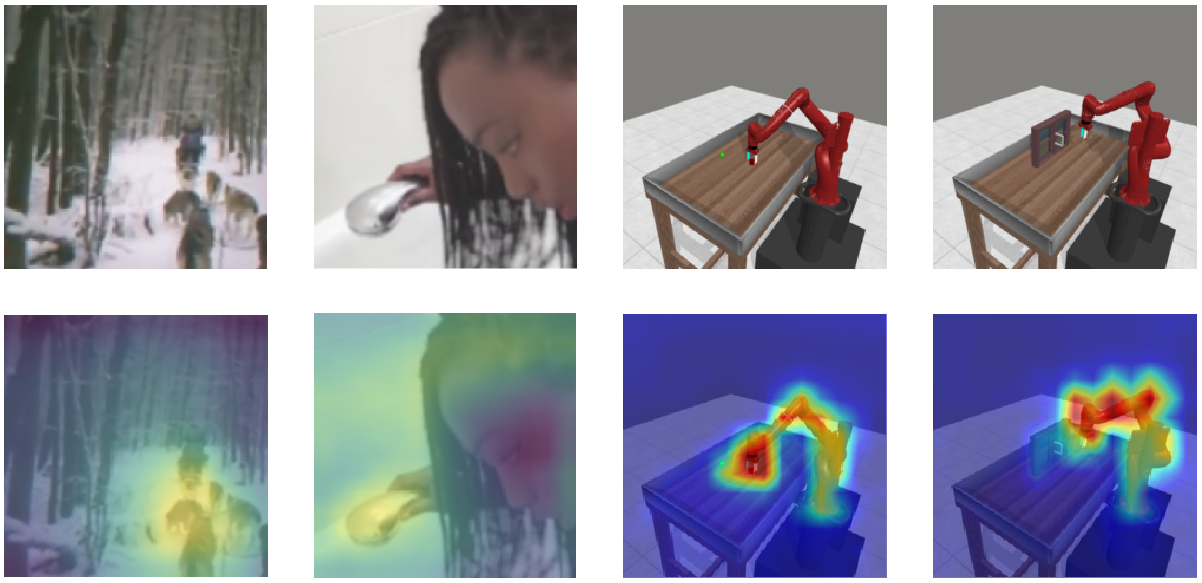
\includegraphics[width=\linewidth]{ieeeconf/figure/vis_attn_cropped.pdf}
    \caption{\textbf{Sampled model attention maps in video prediction}. The language description of top and bottom rows are: ``A person is sled dog racing'' and ``A person is washing hair''. Warmer colors (yellow) indicate higher attention weights, while cooler colors (blue) denote lower attention.}
    \label{fig:vis_attn}
\end{figure}

In Fig.~\ref{fig:vis_attn}, we validate the visual-language grounding capability of LARM by visualizing the cross-attention maps generated by our bidirectional cross-attention given language instructions. The warmer regions (yellow) demonstrate that LARM localizes the task-related moving objects without any bounding-box supervision. This confirms that the model successfully grounds the language intent into the visual space and filters out task-irrelevant background distractors before prediction.





\subsection{Simulation results}
\label{sec:exp_franka}
We validate our model on five long-horizon visuomotor tasks in Franka Kitchen~\cite{franka_kitchen}, a widely adopted continuous control benchmark using a simulated 9-DoF Franka Emika arm. 




\noindent\textbf{Setup.}
As shown in Table~\ref{tab:franka}, we compare our method against three major categories of baselines: standard visual representation models, vision-only predictive models, and vision-language predictive models. To ensure a fair comparison, all downstream policies employ the same standard behavioral cloning (BC) architecture, utilizing the respective frozen backbones.


\begin{table}[!t]
\centering
\caption{\textbf{Pre-training data and supervision for the predictive baselines.} Robot Data indicates whether the representation learner uses robot-domain videos or trajectories during pre-training, and Future Cond. indicates whether future-state prediction is part of the representation objective.}
\begin{tabularx}{\columnwidth}{ l >{\centering\arraybackslash}X >{\centering\arraybackslash}X >{\centering\arraybackslash}X }
\toprule
\textbf{Model} & \textbf{Robot Data} & \textbf{Supervision} & \textbf{Future Cond.} \\
\midrule
MPI        & $\checkmark$ & Bbox, image     & $\times$ \\
LaVA-MAN   & $\checkmark$ & Self-supervised & $\checkmark$ \\

\rowcolor[HTML]{DCD5E0} 
\textbf{Ours}  & \textbf{$\times$}   & \textbf{Self-supervised} & \textbf{$\checkmark$} \\
\bottomrule
\end{tabularx}
\label{tab:dif}
\end{table}



LARM achieves an 81.2\% average success rate, which significantly outperforms standard visual backbones, surpassing MVP \cite{radosavovic2023real} (71.7\%) and Ego4D-trained R3M \cite{nair2022r3m} (69.5\%) by +9.5\% and +11.7\%, respectively. Despite being pre-trained exclusively on human videos without robot embodiment data, LARM successfully generalizes to out-of-domain robotic control, providing a strong affirmative answer to \textbf{Q1}.


% \vspace{-1pt}


Compared to recent vision-language predictive models like LaVA-Man \cite{zhu2025lava} (79.2\%) and MPI \cite{zeng2024learning} (78.9\%), LARM outperforms on complex articulation tasks. For instance, it achieves \textbf{62.0\%} on ``Open microwave'' and \textbf{95.7\%} on ``Flip switch,'' outperforming all predictive baselines. This confirms that explicitly isolating intent-aligned future transitions simplifies downstream policy optimization.


\vspace{-1pt}

% \vspace{-2pt}

Table~\ref{tab:dif} compares pre-training configurations of the predictive models that show similar performance on Franka Kitchen. While MPI and LaVA-Man rely heavily on in-domain robot data, with MPI further requiring expensive fine-grained annotations (e.g., bounding boxes), our method operates without robot data, using self-supervised learning on internet-scale human videos. Despite this strictly scalable setup, LARM systematically outperforms robot data-dependent baselines. By sharing the future-conditioning paradigm with LaVA-Man but removing the reliance on in-domain data, we demonstrate that constrained future prediction is effective for extracting task-relevant physical dynamics from human videos.


% \vspace{-1pt}

\vspace{-1pt}
% \vspace{0.pt}

\subsection{Multi-task generalization on Meta-World}
\label{sec:exp_metaworld}
Franka Kitchen evaluates five tasks that share a single kitchen scene and a common arm configuration. To test whether the intent-aligned residual also helps when a \emph{single} policy must cover heterogeneous scenes, objects and motion primitives, we additionally evaluate on Meta-World MT10~\cite{yu2020meta}, a ten-task multi-task benchmark on a simulated Sawyer arm.

\noindent\textbf{Setup.}
We collect 100 expert demonstrations per task with the benchmark's scripted policies and train a single language-conditioned multi-task policy by offline behavioral cloning, with no reinforcement learning and no online interaction. As in Sec.~\ref{sec:exp_franka}, every backbone is kept frozen and only the action decoder is trained. All methods, including ours, use the identical pooled action decoder, so the only quantity that differs across rows of Table~\ref{tab:metaworld} is the representation supplied to it. We report closed-loop success over 50 episodes per task using an evaluation seed that is disjoint from all demonstration-collection seeds, which prevents the policy from being scored on object configurations it has already seen.

\noindent\rev{\textbf{Visual input.} We render the \texttt{corner2} third-person camera at $224\times224$. The policy consumes a single RGB frame together with a $4$-dimensional proprioceptive state (end-effector position and gripper aperture); no wrist camera, no depth channel and no frame stacking are used. Object positions are randomised by the benchmark at every reset, and the evaluation seed controls that randomisation.}

\begin{table*}[!t]
\centering
\caption{\textbf{Results on Meta-World MT10~\cite{yu2020meta}}. All policies are trained by offline behavioral cloning on 100 expert demonstrations per task with a \emph{frozen} visual backbone, and evaluated over 50 closed-loop episodes per task on a held-out seed disjoint from the demonstration seeds. Backbones denote the largest publicly released checkpoint of each method; ToBo and MPI are only distributed at ViT-Small scale, so this comparison is not scale-matched (see Sec.~\ref{sec:exp_metaworld}). Task names abbreviate the MT10 suite: Drawer-O/C denote drawer open/close and Window-O/C denote window open/close.}
\setlength{\tabcolsep}{3.5pt}
\resizebox{\textwidth}{!}{%
\renewcommand{\arraystretch}{1.05}
\begin{tabular}{llcccccccccc>{\columncolor[HTML]{F5F2F7}}c}
\toprule
\bf Method &
\bf Backbone &
 Reach &
 Push &
 Pick-Place &
 Door &
 Drawer-O &
 Drawer-C &
 Button &
 Peg-Insert &
 Window-O &
 Window-C &
\bf Average \\

\midrule

\rowcolor[HTML]{EFEFEF}
\multicolumn{13}{l}{\textbf{Visual Representation Models}} \\ \midrule
% TODO: DINOv3 (frozen, official) —— 评估 job 44409331 完成后填入这一行
% DINOv3~\cite{simeoni2025dinov3} & ViT-Base  & -- & -- & -- & -- & -- & -- & -- & -- & -- & -- & -- \\
R3M~\cite{nair2022r3m}          & ResNet50  & \bf 50.0 & 32.0 & 2.0 & \bf 100.0 & \bf 100.0 & \bf 100.0 & \bf 100.0 & 26.0 & 90.0 & \bf 100.0 & 70.0 \\
VC-1~\cite{majumdar2023we}      & ViT-Base  & 32.0 & 2.0 & 0.0 & 80.0 & 86.0 & 36.0 & 28.0 & 2.0 & 22.0 & \bf 100.0 & 38.8 \\

\midrule
\rowcolor[HTML]{EFEFEF}
\multicolumn{13}{l}{\textbf{Vision-only Predictive Models}} \\ \midrule
ToBo~\cite{kim2025token}        & ViT-Small & 28.0 & 38.0 & 2.0 & \bf 100.0 & \bf 100.0 & \bf 100.0 & 0.0 & \bf 34.0 & 96.0 & \bf 100.0 & 59.8 \\

\midrule
\rowcolor[HTML]{EFEFEF}
\multicolumn{13}{l}{\textbf{Vision-Language Predictive Models}} \\ \midrule
MPI~\cite{zeng2024learning}     & ViT-Small & 36.0 & 24.0 & 4.0 & 80.0 & \bf 100.0 & \bf 100.0 & 0.0 & 12.0 & 72.0 & \bf 100.0 & 52.8 \\

\rowcolor[HTML]{DCD5E0}
\textbf{Ours} & ViT-Base & 34.0 & \bf 68.0 & \bf 64.0 & \bf 100.0 & \bf 100.0 & \bf 100.0 & \bf 100.0 & 16.0 & \bf 96.0 & \bf 100.0 & \bf 80.8 \\

\bottomrule
\end{tabular}%
}
\label{tab:metaworld}
\end{table*}


\begin{figure}[t]
    \centering
    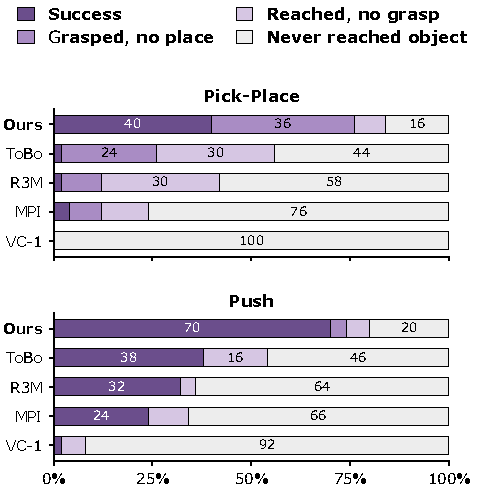
\includegraphics[width=\linewidth]{ieeeconf/figure/failure_stages.pdf}
\caption{\textbf{Where the policies fail on Meta-World.} Every closed-loop episode is assigned to the furthest stage it reaches, using the simulator's \texttt{near\_object}, \texttt{grasp\_success} and \texttt{success} flags; the four outcomes are mutually exclusive and account for all 50 episodes per method and task. The dominant failure of every baseline is not mistimed grasping but never reaching the object at all --- 58\% of episodes for R3M and all 50 for VC-1 on Pick-Place. Conditioning on the predicted future reduces this to 16\%, and the residual failures shift to the strictly later stage of placing an already grasped object. Push requires no grasp, so its \emph{grasped, no place} band is empty by construction.}
    \label{fig:failure_stages}
\end{figure}

\rev{LARM reaches a \textbf{75.6\%} MT10 average, ahead of the strongest baseline R3M~\cite{nair2022r3m} (70.0\%). The aggregate margin is modest, but it is not spread evenly across the suite, and the per-task pattern is the informative part. Six of the ten tasks --- Door, both Drawer tasks, Button and Window-Close --- are at or near saturation for every method that yields a usable representation, and therefore carry no discriminative signal. The entire gap comes from two tasks: ``Pick-Place'' (\textbf{40.0\%} vs.\ at most 18.0\% for any baseline) and ``Push'' (\textbf{70.0\%} vs.\ at most 38.0\%).

These two tasks share a property that the saturated ones lack: the target object moves while the gripper approaches it, so the correct action depends on where the scene is going rather than only on where it currently is. A static embedding is sufficient to replay a memorised opening trajectory, but it under-determines the action once the goal is non-stationary. Conditioning on the intent-aligned residual $\Delta_z$ supplies exactly the missing directional signal, which is why the benefit is invisible on the articulation tasks and decisive on the two dynamic ones. Sec.~\ref{sec:ablation} isolates this effect by removing $\Delta_z$ from our own policy rather than comparing across representations.

The baseline ordering also differs from Franka Kitchen in an informative way. VC-1~\cite{majumdar2023we} (38.8\%), a masked-autoencoding model, transfers markedly worse than the contrastively pre-trained R3M despite a larger backbone, consistent with the view that MAE features are strong for reconstruction but less linearly separable under a frozen-backbone, shallow-decoder protocol.}

\begin{figure*}[t]
\centering
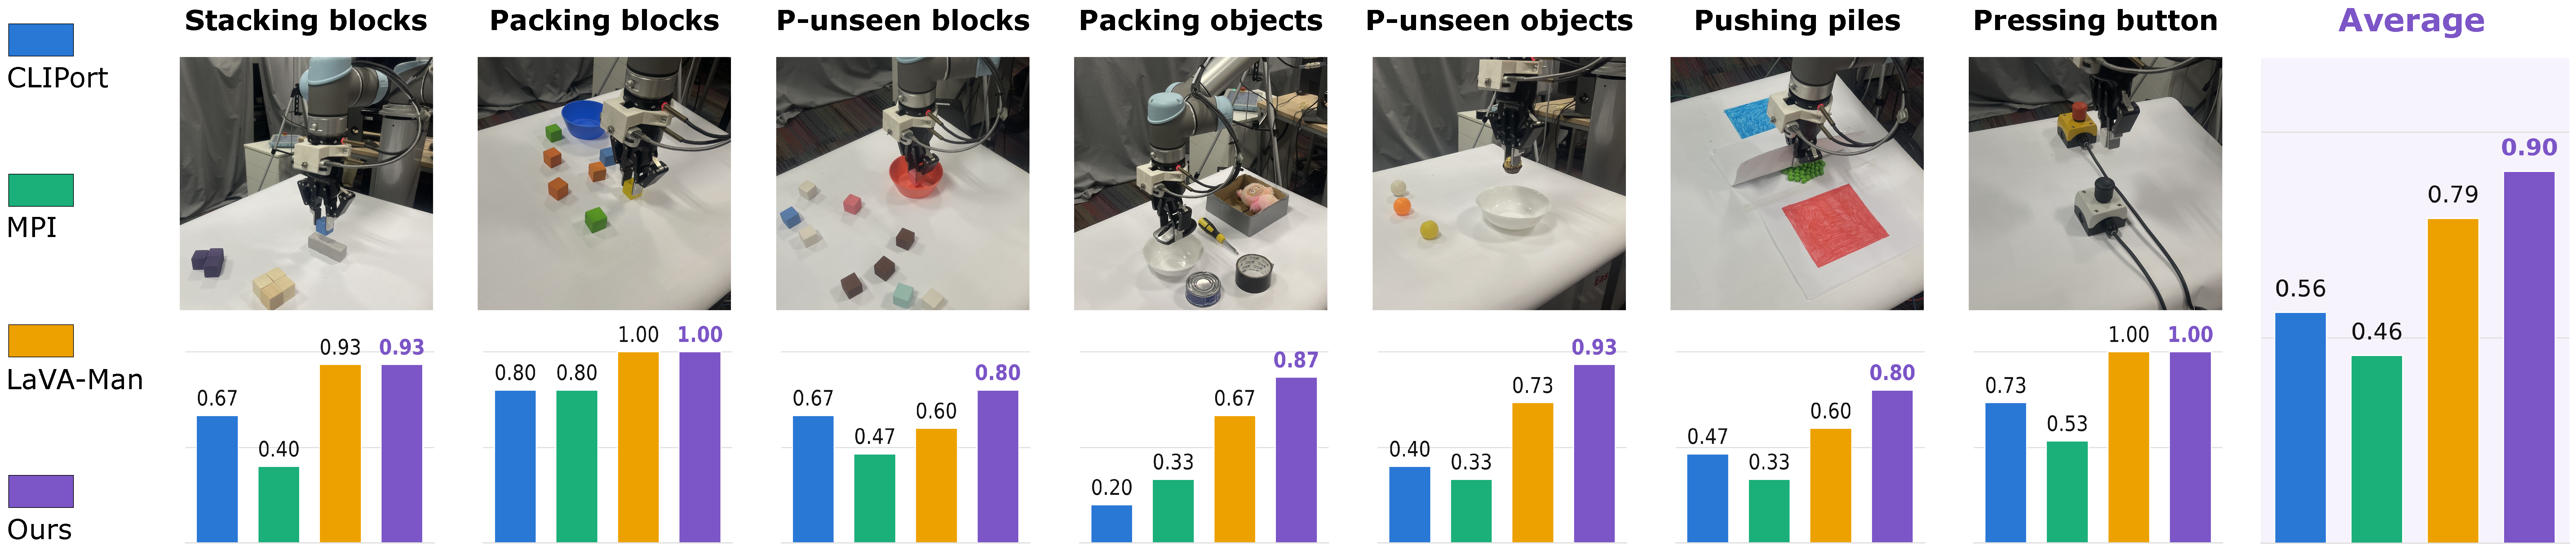
\includegraphics[width=\textwidth]{ieeeconf/figure/arm.pdf}
\caption{ \textbf{Evaluation of real-world multi-task manipulation}. We compare the success rates of our intent-aligned model against CLIPort, MPI, and LaVA-Man across seven language-conditioned tasks. The right panel details our robot hardware setup and the diverse set of experimental objects. Our approach outperforms the baselines in average success rate, exhibiting particularly strong zero-shot generalization on \textit{unseen tasks}. }
\label{fig:robot_results}
\end{figure*}



\begin{figure}[t]  
    \centering
    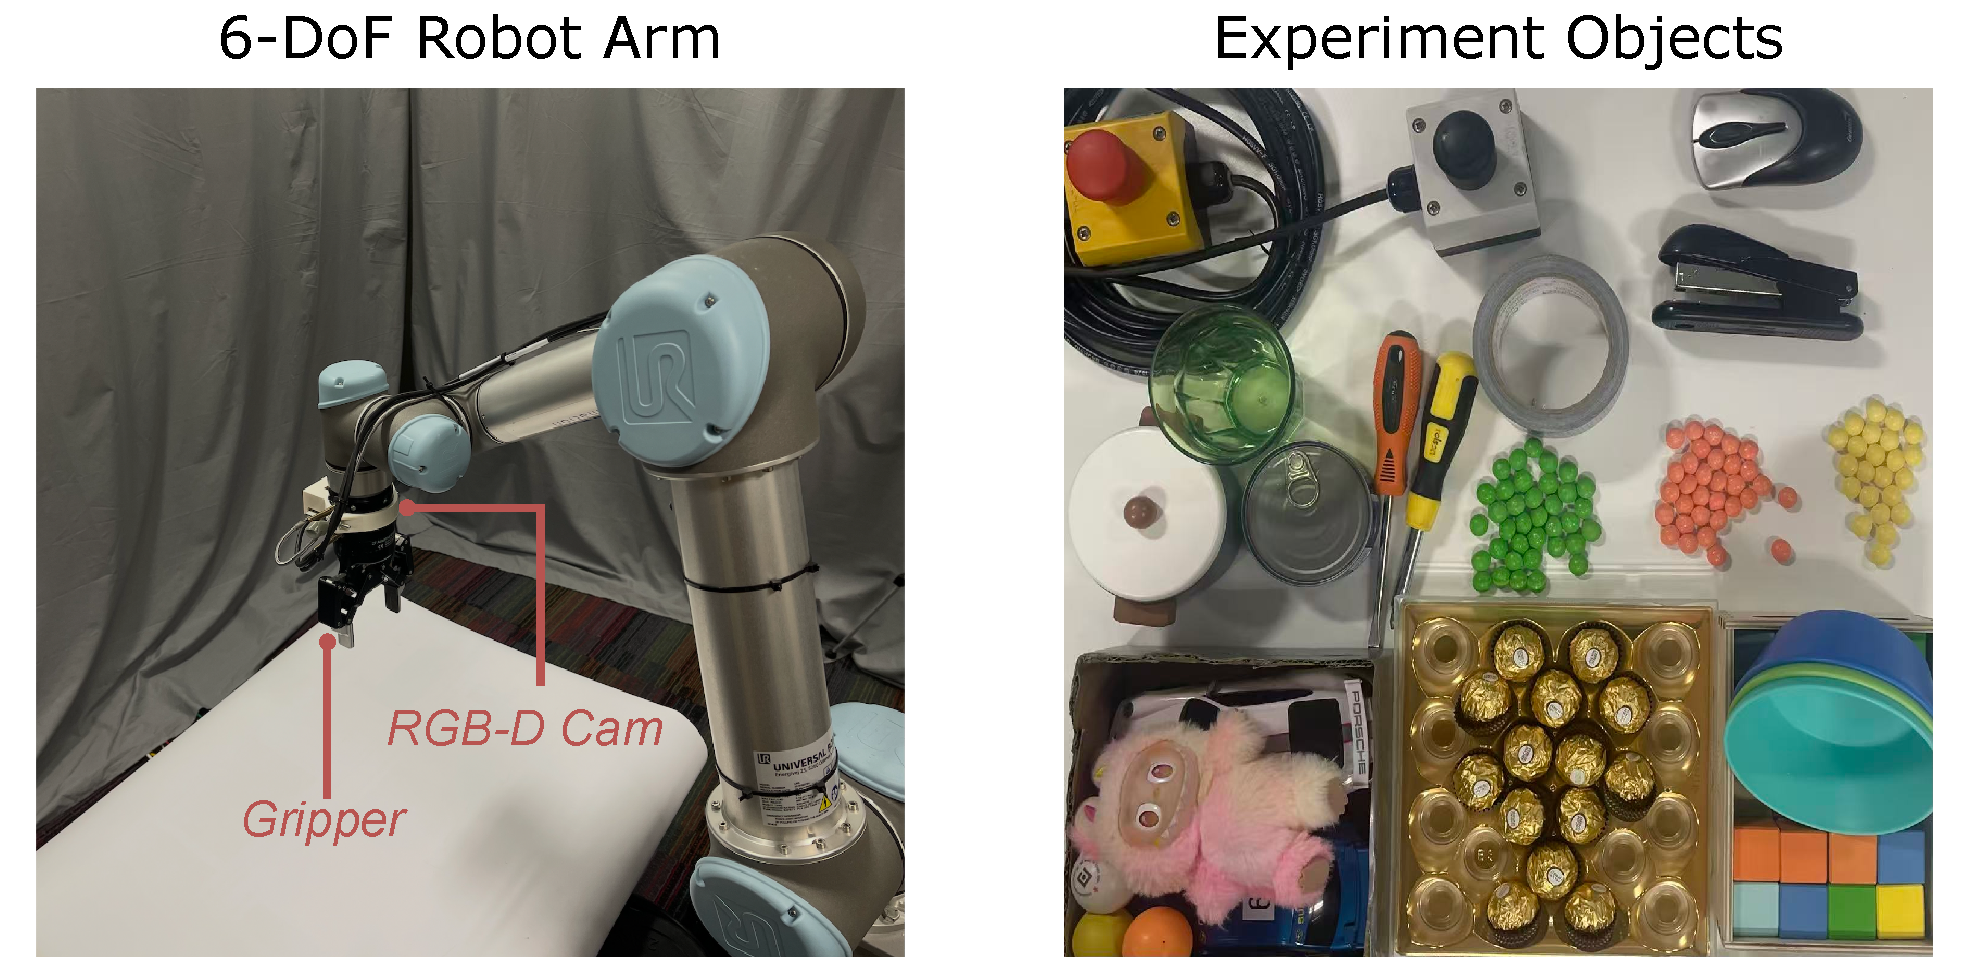
\includegraphics[width=\linewidth]{ieeeconf/figure/setup_cropped.pdf}
    \caption{\textbf{Real-robot experiment setup}. We used various object (left) and a UR5 robot arm with a Robotiq-2F-85 gripper for tabletop manipulation tasks..}
    \label{fig:setup}
\end{figure}



% 



% \begin{table}[!t]
% \Large
% \centering
% \caption{\textbf{Results on Referring Expression Grounding~\cite{voltron}.} Our method outperforms self-supervised methods and is comparable to leading supervised methods. Minimum, Medium and Maximum denote the scenarios categorised according to the level of clutter.} 
% \label{tab:referring}
% \setlength{\tabcolsep}{10pt}
% \resizebox{0.9\columnwidth}{!}{%
% \raisebox{60pt}{
% \begin{tabular}{ccccc}
% % \toprule
% % \multicolumn{5}{c}{\textbf{(Referring Expression Grounding}}\\
% \toprule
% Method     & Minimum    & Medium    & Maximum   & Total          \\ \midrule
% \rowcolor[HTML]{EFEFEF} 
% \multicolumn{5}{l}{\cellcolor[HTML]{EFEFEF}\textit{Supervised pre-training methods}}    \\ \midrule
% MPI~\cite{zeng2024learning}        &  0.94       & \textbf{0.98}   &    0.95        &0.96   \\
% SUGAR~\cite{chen2024sugar}      &  0.98        & 0.97         & \textbf{0.96}     & \textbf{0.97}  \\ \midrule
% \rowcolor[HTML]{EFEFEF} 
% \multicolumn{5}{l}{\cellcolor[HTML]{EFEFEF}\textit{Self-supervised pre-training methods}} \\ \midrule
% R-R3M~\cite{nair2022r3m}      & 0.64                & 0.68              & 0.55              & 0.63           \\
% MVP~\cite{radosavovic2023real}        & 0.51                & 0.52              & 0.40              & 0.49           \\
% CLIP~\cite{radford2021learning}       & 0.67                & 0.77              & 0.60              & 0.68           \\
% Voltron~\cite{karamcheti2023language}    & 0.88                & \textbf{0.97}     & 0.90              & 0.91           \\ 
% LaVA-MAN~\cite{zhu2025lava}       & \textbf{0.99}       & 0.96      & \textbf{0.96}     & \textbf{0.97}  \\
% \rowcolor[HTML]{ECF4FF}
% \bf Ours    & N/A               & N/A     & N/A             & N/A          \\
% \bottomrule
% \end{tabular}%
% % \vspace{-20pt}
% }
% }
% \label{tab:refer}
% \end{table}



\begin{table}[!t]
\centering
\caption{\textbf{Results on Referring Expression Grounding~\cite{karamcheti2023language}.} Our method outperforms self-supervised methods and is comparable to leading supervised methods. Minimum, Medium and Maximum denote the scenarios categorised according to the level of clutter.} 
\label{tab:referring}
\renewcommand{\arraystretch}{1.1} % 稍微增加一点行距，让表格不拥挤
% 使用 tabularx 让表格自动充满单栏 \columnwidth
% l 代表第一列左对齐，后面四个 X 代表自动拉伸并居中
\begin{tabularx}{\columnwidth}{ l *{4}{>{\centering\arraybackslash}X} }
\toprule
Method     & Minimum    & Medium    & Maximum   & Total          \\ \midrule

% 灰色标题行 1
\rowcolor[HTML]{EFEFEF} 
\multicolumn{5}{l}{\textit{Supervised pre-training methods}}    \\ \midrule
MPI~\cite{zeng2024learning}      & 0.94          & \textbf{0.98} & 0.95          & 0.96          \\
SUGAR~\cite{chen2024sugar}       & 0.98          & 0.97          & \textbf{0.96} & \textbf{0.97} \\ \midrule

% 灰色标题行 2
\rowcolor[HTML]{EFEFEF} 
\multicolumn{5}{l}{\textit{Self-supervised pre-training methods}} \\ \midrule
R-R3M~\cite{nair2022r3m}         & 0.64          & 0.68          & 0.55          & 0.63          \\
MVP~\cite{radosavovic2023real}   & 0.51          & 0.52          & 0.40          & 0.49          \\
CLIP~\cite{radford2021learning}  & 0.67          & 0.77          & 0.60          & 0.68          \\
Voltron~\cite{karamcheti2023language} & 0.88     & 0.97 & 0.90          & 0.91          \\ 
LaVA-MAN~\cite{zhu2025lava}      & \textbf{0.99} & 0.96          & \textbf{0.96} & \textbf{0.97} \\

% Ours行，使用之前推荐的高级专业蓝灰色
\rowcolor[HTML]{E8F0F8}
\textbf{Ours}                    & N/A           & N/A           & N/A           & N/A           \\
\bottomrule
\end{tabularx}
\end{table}




\subsection{Real-robot experiment}
\label{sec:real_robot_tabletop}
    % To further assess the robustness of our learned representations and their sim-to-real transferability, we deploy LARM on a physical UR5 robotic arm. Real-world environments introduce severe challenges for representation learning, including varying lighting conditions, complex visual distractors, and partial occlusions—factors that frequently degrade the performance of policies relying on standard static visual features. 


We validate LARM in the real-robot environment using seven tabletop manipulation tasks. 


\noindent\textbf{Setup.} The hardware setup includes a UR5 robotic arm with a Robotiq 2F-85 gripper and an Intel RealSense RGB-D camera capturing a $60 \text{ cm} \times 30 \text{ cm}$ workspace (Fig.~\ref{fig:setup}). To adapt our model to real-world control, we collect 200 language-annotated expert demonstrations. We use this dataset to jointly fine-tune our method and three baselines (CLIPort, MPI, and LaVA-Man) into a single unified multi-task policy, requiring the models to condition their actions on language instructions. To test zero-shot generalization, five colored blocks and five novel objects are strictly excluded from the training data. We evaluate the co-trained policy across seven subtasks: stacking blocks, packing blocks/objects, packing unseen blocks/objects, pushing piles, and pressing buttons. For each subtask, we conduct 5 independent evaluation trials. 

As shown in Fig.~\ref{fig:robot_results}, our method successfully executes the tasks and consistently outperforms the baselines. On average, our model achieves an overall success rate of over 85\%, significantly surpassing the strongest baseline, LaVA-Man ($\sim$70\%), as well as CLIPort and MPI ($\sim$50\%). In Fig.~\ref{fig:affordance_maps}, we demonstrate example pick-and-place affordance maps. Our method exhibits strong zero-shot generalization, achieving a 100\% success rate on ``Packing unseen objects'' (vs. 80\% for LaVA-Man) and an 80\% success rate on ``Packing unseen blocks'' (a 20\% absolute improvement over LaVA-Man). Furthermore, for tasks with complex contact dynamics like ``Pushing piles,'' our method reaches an 80\% success rate, doubling the performance of MPI and LaVA-Man. These results confirm that our intent-aligned pre-training effectively grounds language instructions to visual features, enabling robust continuous control without overfitting.




\begin{figure}[t]  
    \centering
    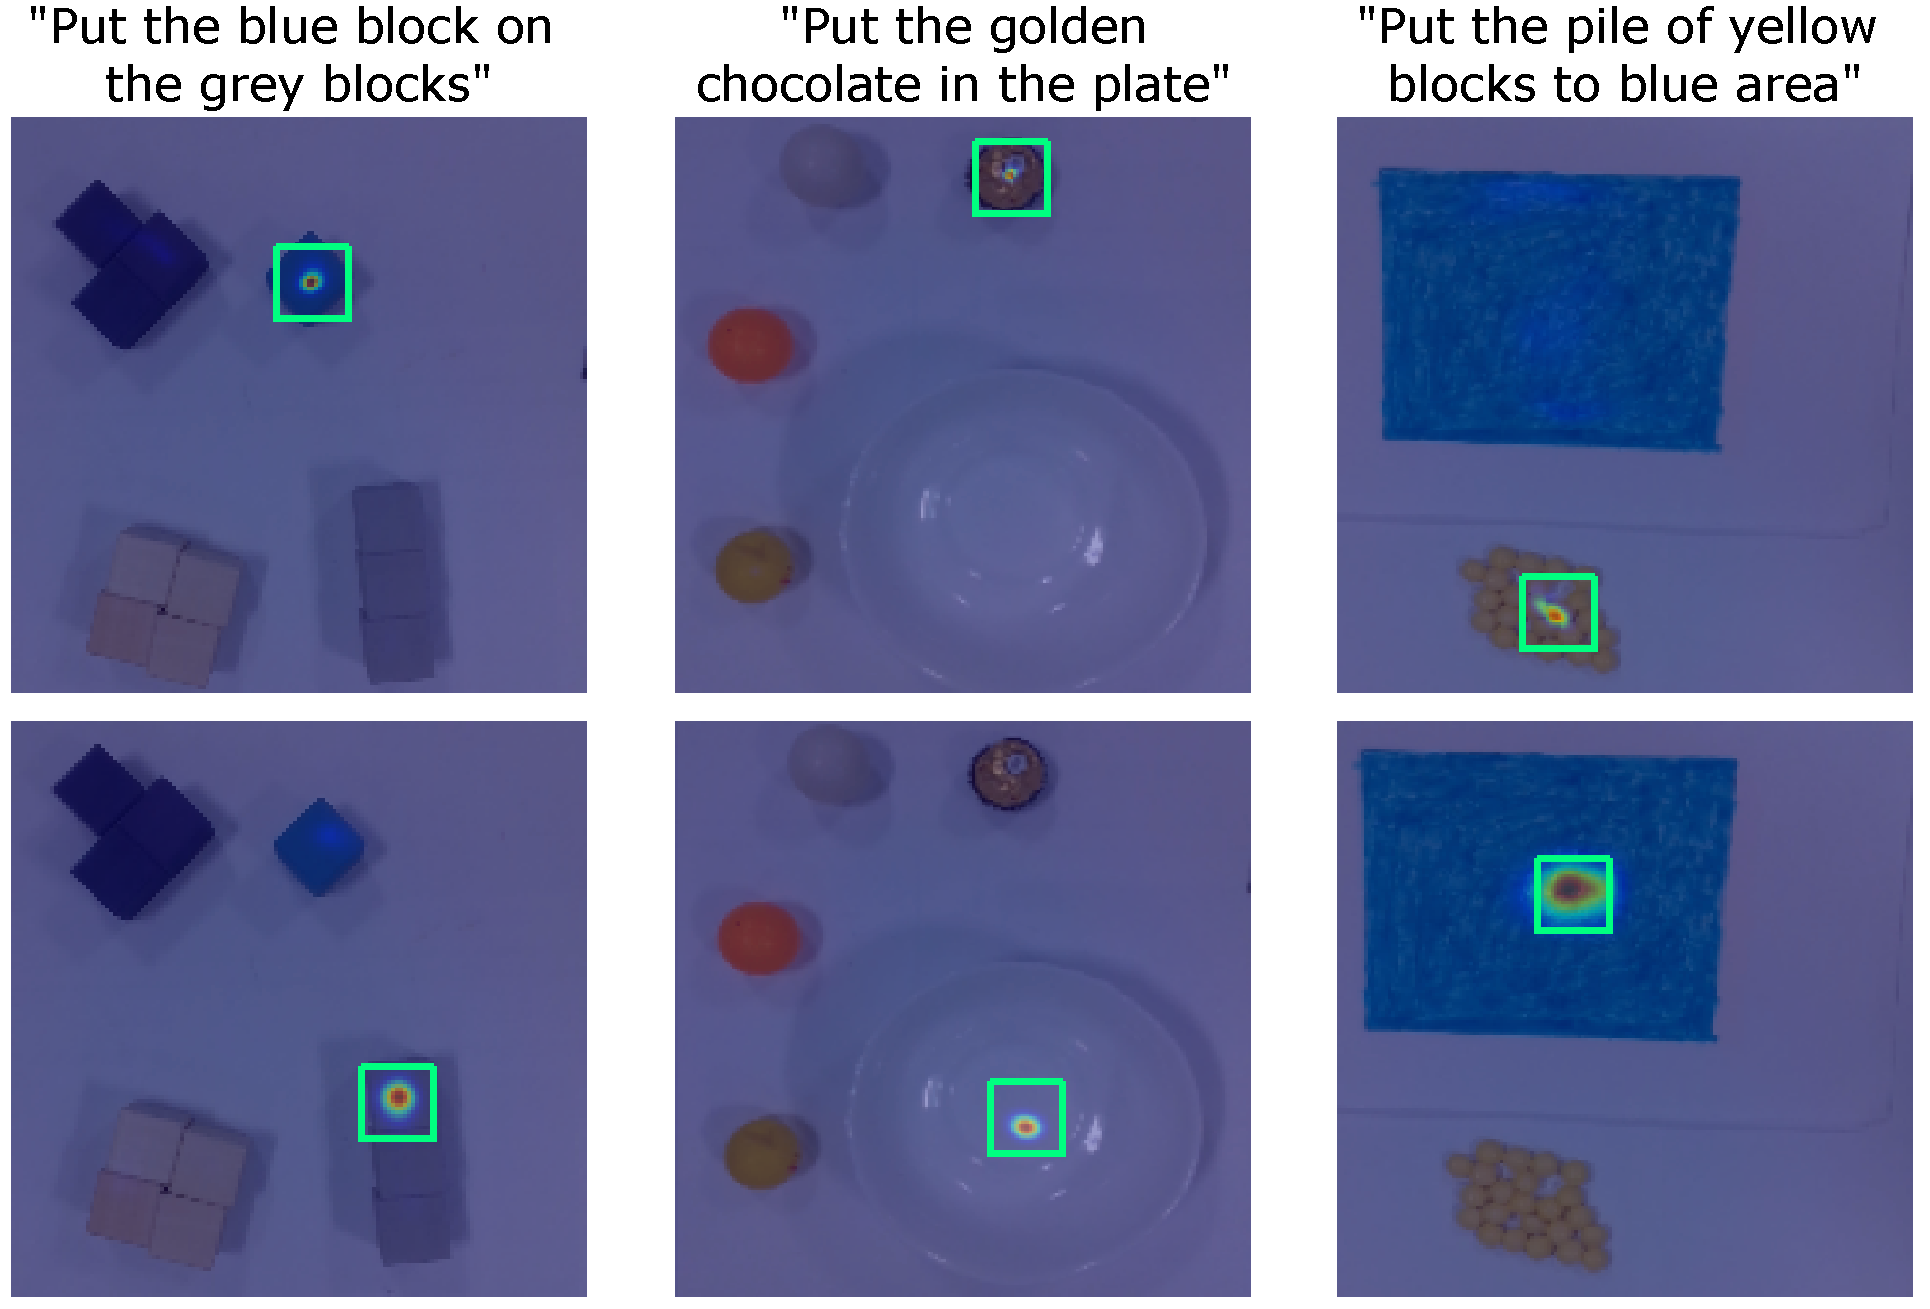
\includegraphics[width=\linewidth]{ieeeconf/figure/aff_cropped.pdf}
\caption{\textbf{Sampled affordance maps.} We obtain the predicted affordance maps of the LARM model at the start and end stages in real-robot tabletop manipulation tasks.}
\label{fig:affordance_maps}
\end{figure}

\subsection{Ablation study}
\label{sec:ablation}
A core contribution of LARM is challenging the standard representation learning paradigm, which typically discards the predictive decoder after pre-training~\cite{he2022masked, nair2022r3m}. We validate the impact of explicitly retaining the intent-aligned predictor by conducting an ablation study on Franka Kitchen~\cite{franka_kitchen}. 

We compare three variants:
\begin{itemize}
    \item \textbf{LARM (Encoder-Only):} The downstream policy is conditioned only on static current visual features $z_t$.
    \item \textbf{LARM (Predictor-Only):} The policy is conditioned exclusively on the predicted future latent state $z_{t+1}$ generated by the predictor.
    \item \textbf{LARM (Full):} The policy is conditioned on both the current state and the explicitly computed intent-aware latent residual: $\pi(z_t, \Delta_z)$.
\end{itemize}


\begin{table}[t]
\centering
\caption{\textbf{Ablation study on latent residuals.} Average closed-loop success on Franka Kitchen and Meta-World MT10. MT10 uses the same frozen-backbone, pooled-decoder protocol as Table~\ref{tab:metaworld}; the Absolute pair variant has not been run on Franka Kitchen.}
\setlength{\tabcolsep}{2.6pt}
\footnotesize
\renewcommand{\arraystretch}{1.03}

\begin{tabular}{@{}llcc@{}}
\toprule
\bf Variant & \bf Input & \bf Franka & \bf MT10 \\
& & \bf Avg. & \bf Avg. \\
\midrule
Encoder-Only & $z_t$ & 74.5 & 57.0 \\
Predictor-Only & $z_{t+1}$ & 75.5 & \bf 79.0 \\
Absolute pair & $z_t,z_{t+1}$ & -- & 75.0 \\
\rowcolor[HTML]{DCD5E0}
\bf Full & \bf $z_t,\Delta_z$ & \bf 81.2 & 75.6 \\
\bottomrule
\end{tabular}
\label{tab:ablation_residual}
\end{table}


As shown in Table~\ref{tab:ablation_residual}, while the \textit{Encoder-Only} variant achieves a competitive average success rate of 74.5\%, it struggles with complex, long-horizon articulation tasks such as ``Open door'' (46.0\%) and ``Open microwave'' (56.3\%). Interestingly, the \textit{Predictor-Only} variant provides only a marginal improvement (75.5\% average), indicating that simply supplying the policy with a raw predicted future state is insufficient for precise motor control. By explicitly computing the actionable latent residual $\Delta_z$, the \textit{Full} LARM model achieves a dramatic $+6.7\%$ absolute improvement over the baseline, reaching an 81.2\% average success rate. This confirms that providing a direct, intent-aligned directional vector effectively simplifies the downstream policy learning objective compared to implicitly forcing the network to infer the difference between $z_t$ and $z_{t+1}$.